% mnras_template.tex
%
% LaTeX template for creating an MNRAS paper
%
% v3.0 released 14 May 2015
% (version numbers match those of mnras.cls)
%
% Copyright (C) Royal Astronomical Society 2015
% Authors:
% Keith T. Smith (Royal Astronomical Society)

% Change log
%
% v3.0 May 2015
%    Renamed to match the new package name
%    Version number matches mnras.cls
%    A few minor tweaks to wording
% v1.0 September 2013
%    Beta testing only - never publicly released
%    First version: a simple (ish) template for creating an MNRAS paper

%%%%%%%%%%%%%%%%%%%%%%%%%%%%%%%%%%%%%%%%%%%%%%%%%%
% Basic setup. Most papers should leave these options alone.
\documentclass[a4paper,fleqn,usenatbib]{mnras}

% MNRAS is set in Times font. If you don't have this installed (most LaTeX
% installations will be fine) or prefer the old Computer Modern fonts, comment
% out the following line
\usepackage{newtxtext,newtxmath}
% Depending on your LaTeX fonts installation, you might get better results with one of these:
%\usepackage{mathptmx}
%\usepackage{txfonts}

% Use vector fonts, so it zooms properly in on-screen viewing software
% Don't change these lines unless you know what you are doing
\usepackage[T1]{fontenc}
\usepackage{ae,aecompl}


%%%%% AUTHORS - PLACE YOUR OWN PACKAGES HERE %%%%%

% Only include extra packages if you really need them. Common packages are:
\usepackage{graphicx}	% Including figure files
\usepackage{amsmath}	% Advanced maths commands
\usepackage{amssymb}	% Extra maths symbols

%%%%%%%%%%%%%%%%%%%%%%%%%%%%%%%%%%%%%%%%%%%%%%%%%%

%%%%% AUTHORS - PLACE YOUR OWN COMMANDS HERE %%%%%

\newcommand{\beq}{\begin{equation}}
\newcommand{\eeq}{\end{equation}}

\newcommand{\tfast}{\texttt{21cmFAST}}

\newcommand{\avg}[1]{\ensuremath{\langle #1 \rangle}}
\newcommand{\CII}{\ensuremath{\text{C~\textsc{ii}}}}
\newcommand{\HII}{\ensuremath{\text{H~\textsc{ii}}}}
\newcommand{\OIII}{\ensuremath{\text{O~\textsc{iii}}}}
\newcommand{\NII}{\ensuremath{\text{N~\textsc{ii}}}}

\newcommand{\Ha}{\ensuremath{\text{H}\alpha}}
\newcommand{\Hb}{\ensuremath{\text{H}\beta}}

\newcommand{\Msun}{\ensuremath{\text{M}_\odot}}
\newcommand{\kpc}{\ensuremath{\text{kpc}}}
\newcommand{\Mpc}{\ensuremath{\text{Mpc}}}
\newcommand{\Myr}{\ensuremath{\text{Myr}}}
\newcommand{\Gyr}{\ensuremath{\text{Gyr}}}
\newcommand{\kms}{\ensuremath{\text{km}\,\text{s}^{-1}}}
\newcommand{\SFR}{\ensuremath{\text{SFR}}}
\newcommand{\yr}{\ensuremath{\text{yr}}}

\newcommand{\hoverMpc}{\ensuremath{h\,\text{Mpc}^{-1}}}

\newcommand{\fid}{\texttt{fid}}
\newcommand{\hot}{\texttt{hot}}
\newcommand{\cold}{\texttt{cold}}

\newcommand{\zst}{\ensuremath{z_{\star}}}
\newcommand{\E}[1]{\mathrm{E}[#1]}
\newcommand{\Var}[1]{\mathrm{Var}[#1]}
\newcommand{\Cov}[2]{\mathrm{Cov}[#1,#2]}

% Please keep new commands to a minimum, and use \newcommand not \def to avoid
% overwriting existing commands. Example:
%\newcommand{\pcm}{\,cm$^{-2}$}	% per cm-squared

%%%%%%%%%%%%%%%%%%%%%%%%%%%%%%%%%%%%%%%%%%%%%%%%%%

%%%%%%%%%%%%%%%%%%% TITLE PAGE %%%%%%%%%%%%%%%%%%%

% Title of the paper, and the short title which is used in the headers.
% Keep the title short and informative.
\title[The transition redshift as an EoR probe]{The transition redshift as a probe of reionization}

% The list of authors, and the short list which is used in the headers.
% If you need two or more lines of authors, add an extra line using \newauthor
\author[A. Beane et al.]{
Angus Beane,$^{1}$\thanks{E-mail: angus.beane@cfa.harvard.edu}
Adam Lidz,$^{2}$
Kana Moriwaki,$^{3}$
and others
\\
% List of institutions
$^{1}$Center for Astrophysics {\normalfont |} Harvard \& Smithsonian, 60 Garden Street, Cambridge, MA 02138, USA\\
$^{2}$Department of Physics \& Astronomy, University of Pennsylvania, 209 South 33rd Street, Philadelphia, PA 19104, USA\\
$^{3}$Department of Physics, The University of Tokyo, 7-3-1 Hongo, Bunkyo, Tokyo 113-0033, Japan
% $^{2}$Center for Computational Astrophysics, Flatiron Institute, 162 5th Avenue, New York, NY 10010, USA\\
}

% These dates will be filled out by the publisher
\date{Accepted XXX. Received YYY; in original form ZZZ}

% Enter the current year, for the copyright statements etc.
\pubyear{2019}

% Don't change these lines
\begin{document}
\label{firstpage}
\pagerange{\pageref{firstpage}--\pageref{lastpage}}
\maketitle

% Abstract of the paper
\begin{abstract}
The early stages of the Epoch of Reionization (EoR), probed by the 21~cm line,
are sensitive to the detailed formation of the first galaxies. An important
transition occurs on large scales at $z\sim10$, when the 21~cm field changes
from being positively correlated with the density field to being negatively
correlated. The redshift at which this occurs (the ``transition redshift'') is
in principle measurable if the 21~cm field can be cross-correlated with a
tracer of the density field (such as galaxies or a line intensity map) at that
high redshift. Since the transition redshift is derived from a
cross-correlation, it naively depends on the structure of the 21~cm field and
the tracer field. However, we show that on large scales the transition
redshift is independent of the structure of the tracer field. We verify this
in simulations by assuming a simple model for a mock Ly$\alpha$ intensity
mapping survey. By considering a joint measurement between the Square
Kilometre Array and the Cosmic Dawn Intensity Mapper, we show that the
transition redshift is measurable up until about $z\sim x$. Being derived from
a cross-correlation, the transition redshift is less impacted by foreground
contamination currently inhibiting 21~cm auto-spectrum measurements.
Therefore, the transition redshift is an interesting probe of the early stages
of the EoR, and its detectability and interpretability deserve further study.
\end{abstract}

% Select between one and six entries from the list of approved keywords.
% Don't make up new ones.
\begin{keywords}
cosmology: theory -- dark ages, reionization, first stars -- large-scale
structure of Universe
\end{keywords}

%%%%%%%%%%%%%%%%%%%%%%%%%%%%%%%%%%%%%%%%%%%%%%%%%%

%%%%%%%%%%%%%%%%% BODY OF PAPER %%%%%%%%%%%%%%%%%%

\section{Introduction} \label{sec:intro}
The redshifted 21~cm line contains a great deal of information about the
structure and evolution of the Epoch of Reionization (EoR). Once measured at
$z\sim6\textup{--}12$, it should reveal the nature of the formation of the
first stars, galaxies, and black holes, as well as the large-scale structure
of the Universe at high redshift \citep{2013fgu..book.....L}. While
instruments have reached the sensitivity necessary to detect the signal during
the EoR, issues of foreground contamination and instrumental artifacts have so
far prevented the success of such efforts. Only upper limits have been placed
on the amplitude of the 21~cm fluctuations \citep[e.g.][]{2013MNRAS.433..639P,
2014PhRvD..89b3002D, 2016ApJ...833..102B, 2017ApJ...838...65P}.

Because of the great difficulties confronting 21~cm auto-spectrum
measurements, the prospect of measuring 21~cm in cross-correlation with
another tracer of large-scale structure, such as galaxies. The galaxy field
will only correlate with the cosmological 21~cm signal, and the foregrounds
will not contribute to the mean signal (though they will make the measurement
noisy, and so some foreground subtraction is still necessary).

The 21~cm-galaxy cross-correlation was first explored by
\citet{2007MNRAS.375.1034W} in the context of using Ly$\alpha$-emitters to
distinguish between ``inside-out'' and ``outside-in'' reionization scenarios.
However, this technique is limited to the late stages of reionization since
Ly$\alpha$-emitters are obscured by neutral hydrogen even slightly earlier
into the EoR \citep[e.g.][]{2006ApJ...648....7K}. \citet{2007ApJ...660.1030F}
expanded upon this by considering a general galaxy survey. It was later shown
that the scale at which the cross-correlation goes from negative to zero (the
``turnover scale'') provides a tracer of the bubble size. However, the precise
turnover scale also depends on the properties of the selected galaxy sample,
with turnover happening on larger scales if only more massive galaxies can be
detected \citep{2009ApJ...690..252L}. A number of authors have studied this
cross-correlation in the context of detectability of the anti-correlation on
large scales \citep{2013MNRAS.432.2615W, 2016MNRAS.457..666V,
2017ApJ...836..176H}, and its dependence on the details of the EoR
\citep{2014MNRAS.438.2474P}.

In addition to the cross-correlation between 21~cm and galaxies, the
cross-correlation between 21~cm and intensity maps has been investigated in an
analogous fashion. Line intensity mapping experiments aim to measure the
large-scale structure of emission in a certain line, and is easier to perform
over a large area at high redshift than a galaxy survey. Current targets
include [\CII], CO, Ly$\alpha$, and H$\alpha$ \citep[for a recent review,
see][]{2017arXiv170909066K}. Another intriguing possible line is [\OIII]
$88\,\mu \text{m}$ \citep[e.g.][]{2018MNRAS.481L..84M}, in which a lensed
$z=9.1$ galaxy has recently shown to be exceptionally bright
\citep{2018Natur.557..392H}.

This cross-correlation was first studied with the CO rotational lines
\citep{2011ApJ...741...70L}, and then the [\CII] \citep{2012ApJ...745...49G}
and Ly$\alpha$ lines \citep{2013ApJ...763..132S}. The possibility of using the
cross-bispectrum the 21~cm and [\CII] fields has been explored
\citep{2018ApJ...867...26B}, along with combining the three cross-spectra with
a 21~cm, [\CII], and [\OIII] overlap \citep{2019ApJ...874..133B}. Because the
transition redshift is typically $\z_{\star} \sim 10$, it is unclear how much
metal enrichment will have occurred by this early time. 

In the case of either galaxies or emission lines, it is expected that the two
are positively correlated at the very beginning of the EoR (though the
emission lines may be very weak due to the lack of significant metal
enhancement). This is because the densest regions host the most mass and
therefore 21~cm emission and galaxy populations. However, the densest regions
will also ionize first {\bf cite something}, and after some time 21~cm and
galaxies will become negatively correlated. We refer to the redshift at which
this transition occurs at a fixed $k$ as the ``transition redshift''
$z_\star(k)$, assuming that only one such zero exists. In other words, the
cross-correlation at $k$ vanishes at $z=z_{\star}(k)$.

In this work we investigate to what extent the transition redshift is
dependent upon the galaxy sample used to define it. We assume a galaxy catalog
selected using an [\OIII] emitter survey. In particular, we are interested in
how $z_\star$ changes as we vary the parameters of the [\OIII] luminosity-mass
relation for a fixed halo catalog.

\section{Methods} \label{sec:methods}
\subsection{The transition redshift} \label{ssec:ztran_def}
The transition redshift $\zst(k)$ is defined by a field $x$ which traces the
density field on large scales and the condition that
\beq \label{eq:ztran_def}
P_{21,x}(k, \zst(k)) \equiv 0\text{.}
\eeq
If more than one such \zst{} exists, then we choose the lowest one where
$P_{21,x}$ last transitioned from positive to negative.

\subsection{21cmFAST} \label{ssec:tfast}
We generate realizations of the 21~cm field for our different EoR models using
the publicly available code \tfast{}
v1.3\footnote{\url{https://github.com/andreimesinger/21cmFAST}, commit:
\texttt{42e7566}}. Spin temperature fluctuations are computed and the
excursion set approach is used to identify the ionized regions
\citep{2011MNRAS.411..955M}. Rather than using the mean collapsed fraction, we
use the halo field to compute the ionization and 21~cm fields, since we are
interested in the evolution at early redshifts where the Poisson statistics of
the halo field can be important.

The parameters used in our \tfast{} runs are as folows. The minimum halo mass
contributing to the ionizing budget is $10^{8}\,\Msun$. The \HII{} efficiency
factor ($\zeta$) is set to $10$. The maximum smoothing scale for the
ionization field $R_{\text{max}}$ (loosely referred to as the ``mean-free
path'') is set to $30\,\Mpc$, though this quantity has almost no effect on the
early stage of the EoR. We set the fraction of baryons converted to stars
($f_\star$) to be $0.1$. We ignore redshift-space distortions for convenience.
All other parameters are set to their default values, except for the heating
parameter discussed in the next paragraph. The exact parameter files are given
in the github repository associated with this work (see the Supplementary
Material).

Our three different models for the EoR differ in the efficiency of their
heating, controlled by the number of X-ray photons per solar mass in galaxies
($\zeta_X$). Our fiducial model (\fid{}) is the default value
$\zeta_X=2\times10^{56}$, while our ``hot'' and ``cold'' models (\hot{} and
\cold{}) set $\zeta_X=10^{57}$ and $5\times10^{55}$, respectively. The average
$\delta T_b$ signal is shown in \textbf{some figure}, which shows
\textbf{something}. Note that none of these models account for the recent
claimed detection by the EDGES group of an extremely deep absorption trough at
$z\sim17$ \citep{2018Natur.555...67B}. If confirmed, though, that detection
would indicate an extremely low gas temperature at $z\sim17$, which would
favor larger amplitudes of the spin temperature fluctuations at $z\sim10$,
unless heating were extremely efficient after $z\sim17$. {\bf don't know how I
feel about the last sentence}

We generate the halo field using the included halo finder in \tfast{}. This
halo finder is a remnant of an earlier version of the code
\citep{2007ApJ...669..663M} and is typically unused in standard
configurations. It is based upon the ``peak-patch'' algorithm for halo finding
introduced by \citet{1996ApJS..103....1B}.

\subsection{Intensity mapping} \label{ssec:oiii_int_map}
In order to model the relation between luminosity ($L$) and
halo mass, we follow \citet{2019ApJ...874..133B}. Specifically, we assume that
the mean luminosity of a halo of mass $M$ is,
\beq \label{eq:lum_mass_relation}
\avg{L}(M) = L_0 \left[ \frac{M}{M_0} \right]^{\alpha}\text{,}
\eeq
where $L_0/M_0^{\alpha}$ is set to match the total average intensity of
the line at that redshift and $\alpha$ is the power-law index. We then draw the
luminosity of each halo from a lognormal distribution of mean $\avg{L}(M)$ and
scatter $\sigma$. Once the average intensity is fixed (which we assume so),
this is a two-parameter model ($\alpha$ and $\sigma$) of the
luminosity-mass relation. In practice, the average intensity of the field only
enters in the detectability calculation, so we instead work in the convenient
units where $L_0=1$ and $M_0=10^{10}\,\Msun$.

We assign a luminosity to each halo according to this prescription. An
important consideration is that we have not specified which line we are
working with. In detail, the relationship between a halo and it's luminosity
is a complicated function of the state of the interstellar medium of the
hosted galaxy, which can depend upon a number of both deterministic and
stochastic quantities. Our model crudely attempts to account for this by
including some random scatter, but will ultimately be a rough description of
reality.

{\bf Some words justifying why our simple model will extend to more
complicated luminosity-halo relations.}

\section{Results} \label{sec:results}
\subsection{The transition redshift} \label{ssec:ztran_results}

\begin{figure*}
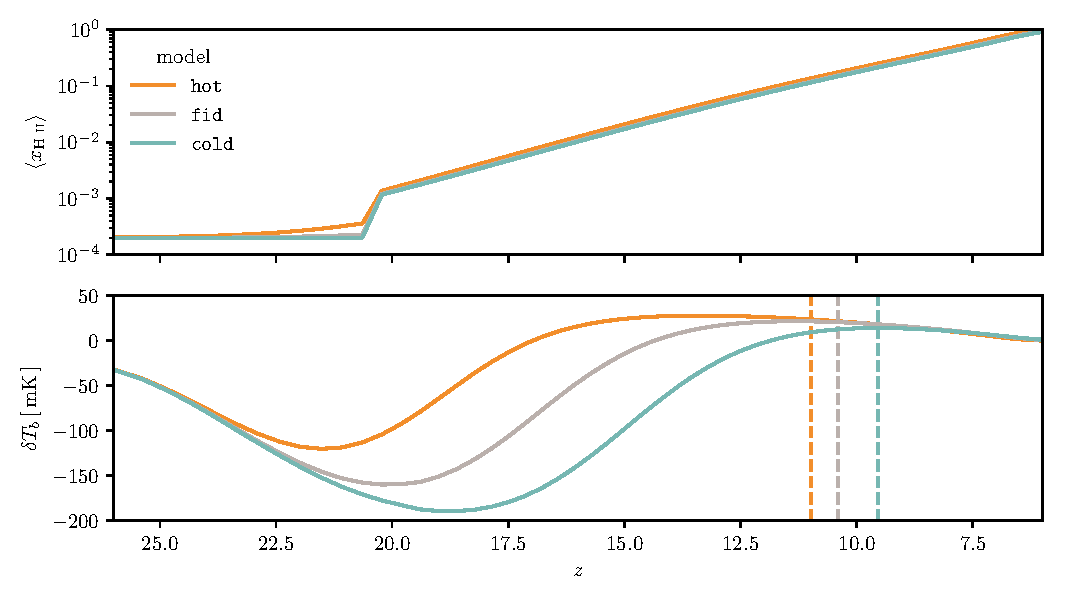
\includegraphics[width=\textwidth]{plots/aveTb_nf.pdf}
\caption{A summary of the ionization and heating history of our three EoR
models: \hot{}, \fid{}, and \cold{}. \textit{Upper}: the ionization history of
each model, showing that reionization begins ($\avg{x_{\HII}}\sim0.01$) at
$z\sim16$ and ends at $z\sim6$ in each model. In detail the ionization
histories are slightly different, but not drastically. \textit{Lower}: the
heating history of each model, showing the strong differences in the monopole
signal. The transition redshift \zst{} (defined where $P_{21,\delta}(\zst{}) =
0$) for each model is shown as a vertically dashed line. We see that models in
which heating is more efficient have an earlier \zst{}.}
\label{fig:aveTb_nf}
\end{figure*}

\subsection{The halo field}
{\bf If we switch to LIM I think this section should be scrapped, except
showing ztran vs k but using LIM and density instead of halos}

We first investigate the dependence of the transition redshift as defined by
the halo field. Fig.~\ref{fig:ztran_vs_k} shows the transition redshift
defined by the 21~cm\,--\,density cross-power spectrum (see
Eq.~\ref{eq:ztran_def}) as a function of $k$. The three models considered in
this work are shown in orange, gray, and teal (\hot{}, \fid{}, and \cold{},
respectively).

Fig.~\ref{fig:ztran_vs_k} shows that \zst{} is only weakly a function of $k$. 

\begin{figure}
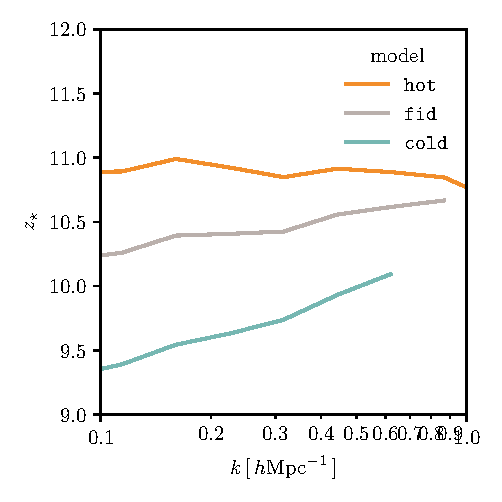
\includegraphics[width=\columnwidth]{plots/ztran_vs_k.pdf}
\caption{The transition redshift ($\zst$) as defined by cross-correlating with the
density field (solid lines) and all resolved halos (dashed lines, $M\gtrsim
5\times10^9\,\Msun$), for our three different EoR models (\hot{}, \fid{}, and
\cold{}). We see that \zst{} is only a mild function of $k$ for the three
models, with slightly stronger dependence as the heating of the model
decreases. The most dependence comes in the \cold{} model, where \zst{}
changes by $\sim7\,\%$ from $k=0.1$ to $0.6\,\hoverMpc$. {\bf Some words for
why cold and fid cut off at some k}}
\label{fig:ztran_vs_k}
\end{figure}

\begin{figure}
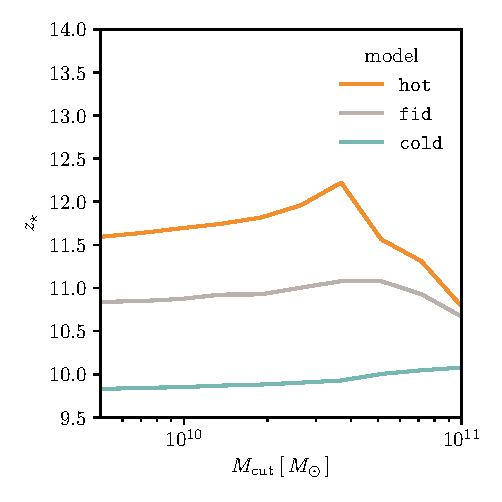
\includegraphics[width=\columnwidth]{plots/ztran_vs_Mcut.pdf}
\caption{The transition redshift (\zst) as defined by cross-correlating with
the halo field for our three different EoR models (\hot{}, \fid{}, and
\cold{}) as a function of the cut-off mass. The cross-correlation is only made
between the 21~cm field and all halos with masses $M>M_{\text{cut}}$. One can
see that for the \fid{} and \cold{} models, \zst{} is only mildly a function
of $M_{\text{cut}}$ below a certain cut-off mass ($\sim10^{10.5}\,\Msun$ in
both models). In other words, as long as a galaxy survey is deep enough so as
to resolve a sufficient number of galaxies, the \zst{} is not dependent on the
depth of the survey. The \hot{} model shows more dependence, but this may be
due to sampling noise due to the smaller number of such halos at the higher
\zst{} typical for the \hot{} model.}
\end{figure}

\subsection{Line-intensity mapping} \label{ssec:lim}
We now turn to understanding how \zst{} depends on the parameters of our
generic line-intensity mapping field: the slope ($\alpha$) and lognormal
scatter ($\sigma$). See \S~\ref{ssec:oiii_int_map} for more details of the
construction of the field.

In Fig.~\ref{fig:ztran_vs_alpha_sigma} we plot \zst{} as a function of each of
these parameters\,--\,$\alpha$ and $\sigma$. We see that \zst{} is remarkably
insensitive to the value of either of these parameters, with some small
deviation as a function of $\alpha$. The \hot{}, \fid{}, and \cold{} models
only vary by a total of $1.2\%$, $0.56\%$, $0.52\%$ with respect to $\alpha$,
and $0.070\%$, $0.10\%$, and $0.11\%$ with respect to $\sigma$, respectively.

\begin{figure*}
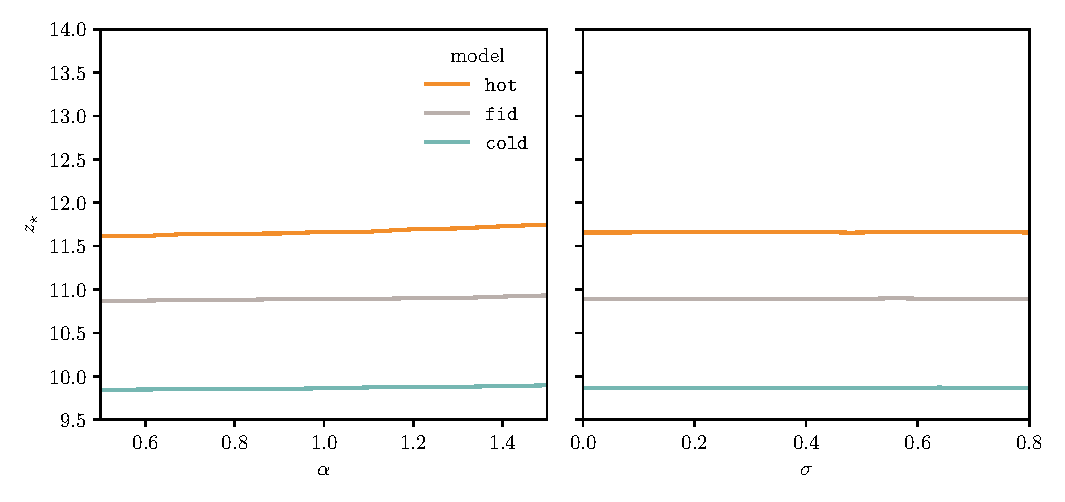
\includegraphics[width=\textwidth]{plots/ztran_vs_alpha_sigma.pdf}
\caption{The transition redshift (\zst) defined by cross-correlating with a
generic two-parameter intensity mapping field. The parameter $\alpha$ sets the
slope of the luminosity-mass relation and the parameter $\sigma$ sets the
lognormal scatter in this relation (see \S~\ref{ssec:oiii_int_map}). The
\hot{}, \fid{}, and \cold{} models only vary by a total of $1.2\%$, $0.56\%$,
$0.52\%$ with respect to $\alpha$, and $0.070\%$, $0.10\%$, and $0.11\%$ with
respect to $\sigma$, respectively. Clearly \zst{} varies only with the
structure of the 21~cm field, and is thus an excellent probe of reionization.}
\label{fig:ztran_vs_alpha_sigma}
\end{figure*}

\section{Detectability}
Up to this point, we have not been specific about which galactic emission line
one might consider using to measure \zst{}\,--\,in fact, our entire formalism
could be executed using a galaxy survey, if one with sufficient redshift
accuracy and depth could be executed. While it will not be possible for a
traditional galaxy survey to extend to $z\sim10$ in the near future, it may be
possible to execute a survey of line-emitting galaxies, e.g., with
[\OIII]-emitters \citep{2018MNRAS.481L..84M, 2019arXiv190610863M}.

In this work we will consider the prospect of performing intensity mapping
measurements of the H$\alpha$ line using the proposed, space-based Cosmic Dawn
Intensity Mapper (CDIM) \citep{2019arXiv190303144C}. CDIM is an infrared
telescope with an $83\,\text{cm}$ dish capable of measuring $R=300$ spectra
from wavelengths $0.75\,\mu\text{m}$ to $7.5\,\mu\text{m}$. Therefore, CDIM
will be able to measure the H-$\alpha$ line ($656\,\text{nm}$) from $z=0.14$
to $10.4$ and the H-$\beta$ line ($486\,\text{nm}$) from $z=0.54$ to $14.4$,
so long as there is a detectable signal. CDIM will execute a wide, medium, and
deep survey of $311$, $31.1$, and $15.6\,\text{deg}^2$, respectively. However,
only the medium survey's field will overlap with 21~cm experiments (HERA and a
deep field from SKA1-LOW). Therefore we will only consider the medium survey.

We choose to study the H-$\alpha$ and H-$\beta$ lines since the uncertainty
regarding their total intensity at $z\sim10$ should be less uncertain than for
lines that require metal enrichment such as [\CII], [\OIII], or [\NII], since
the total metal enrichment of the universe is quickly declining at these high
$z$

We assume a linear relationship between H-$\alpha$ luminosity and star
formation rate \citep{1998ARA&A..36..189K}:
\beq \label{eq:LHalpha_SFR}
\begin{split}
L_{\Ha} &= 3.29\times10^{7} \left(\frac{\SFR}{1\,\Msun\,\yr^{-1}}\right) L_{\odot} \\
        &\equiv L_{0,\Ha} \left(\frac{\SFR}{1\,\Msun\,\yr^{-1}}\right)
\end{split}
\eeq
This relation is based on a Salpeter IMF and is calibrated towards local
galaxies. As discussed in \citet{2019MNRAS.487.5902K}, the reality of
$z\sim10$ galaxies may be slightly different\,--\,the IMF may be more top
heavy, and the metal-poor nature of a typical star will naturally produce more
ionizing photons. However, the escape of ionizing photons may be more
efficient at higher redshift, and the conventional relation assumes no escape.
\citet{2019MNRAS.487.5902K} provide a slightly shallower fitting form for the
$L_{\Ha}-\SFR$ relation based upon their simulations, but we choose to use the
conventional relation here.

We use a fitting formula for the SFRd calibrated upon galaxies from $z=0$ to
$8$ \citep{2014ARA&A..52..415M}
\beq \label{eq:sfrd}
\psi(z) = 0.015 \frac{(1+z)^{2.7}}{1+\left[(1+z)/2.9\right]^{5.6}}\,M_{\odot}\yr^{-1}\Mpc^{-3} \text{.}
\eeq
The comoving emissitivity of the \Ha{} line can then be readily computed as,
\beq \label{eq:Ha_emiss}
\epsilon_{\Ha}(z) = L_{0,\Ha} \psi(z)\text{.}
\eeq
The average specific intensity can be computed from the comoving emissitivity
as \citep{2011ApJ...741...70L,2013ApJ...768...15P},
\beq \label{eq:int_from_em}
\avg{I_{\Ha}}(z) = \frac{\epsilon_{\Ha}(z)}{4\pi\nu_{\text{rest},\Ha}} \frac{c}{H(z)}
\eeq

The variance per mode of the cross-spectrum between the 21~cm field and a line
$i$ is given by \citep[e.g.][]{2007ApJ...660.1030F}
\beq \label{eq:var_xps}
\Var{P_{21,i}} = P_{21,i}^2 + 
                                  P_{21,\text{tot}} P_{i,\text{tot}}\text{,}
\eeq
where $P_{21,\text{tot}} = P_{21,21} + N_{21}$, where $N_{21}$ is the total
noise contribution. $P_{i,\text{tot}}$ is defined similarly.

In detail the surface brightness sensitivity will have a frequency-dependent
structure, but for $z\sim9$ to $10$, it is reasonable to assume a
conservative, constant value of
$\sigma_{\Ha}\sim4\times10^4\,\text{Jy}/\text{sr}$ for the medium survey. To
convert the surface brightness sensitivity to a power spectrum noise, we simply
write,
\beq \label{eq:ps_}
N_{\Ha} = \sigma_{\Ha}^2 V_{\text{voxel}}\text{,}
\eeq 
where $V_{\text{voxel}}$ is the comoving volume of one voxel. To compute this
we use the fact that CDIM will have $1''$ pixels and a resolution of $R=300$.

For
$N_{21}$, we assume that $N_{21} = P_{21,21}(k=0.1\,\text{Mpc}^{-1})$, a
reasonable approximation given that HERA-350 will image some large scale modes
\citep{2017PASP..129d5001D}, as discussed previously \citep{2018ApJ...867...26B}.

The number of modes is given by,
\beq \label{eq:nmodes}
N_m = \frac{4\pi k^2 \delta k}{V_{\text{fund}}}\text{,}
\eeq
where $\delta k$ is the width of the $k$-bin and $V_{\text{fund}}$ is the
volume of a fundamental mode. We assume a square survey area, and so this is
given by,
\beq \label{eq:fund}
V_{\text{fund}} = \frac{(2 \pi)^3}{L_{\perp}^2 L_{\parallel}}\text{,}
\eeq
where $L_{\perp}$ is the  and $L_{\parallel}$ is the comoving length of the
redshift extent of the bin. The optimal redshift binning is not entirely
clear, since the observational target is not the power spectrum. We assume a
redshift bin of $\Delta z = 0.03$, which is smaller than the expected error we
compute on \zst{}, and so is not an unreasonable choice. We assume a $k$-bin
of fairly large width, from $k=0.1$ to $0.4\,\Mpc^{-1}$.

By expanding $P_{21,\Ha}$ as a linear function about \zst{}, we can estimate the
error on \zst{} by
\beq \label{eq:error_on_zst}
\Var{\zst} = \left(\left.\frac{\partial P_{21,\Ha}}{\partial z}\right|_{\zst}\right)^{-2} \Var{P_{21,\Ha}}\text{,}
\eeq
where ${\partial P_{21,\Ha}}/{\partial z}$ is computed numerically.


\section{Conclusions} \label{sec:conclusions}

The conclusions.

\section*{Acknowledgements}

The Acknowledgements section.

\section*{Utility}
Some links to be saved for later

Ly$\alpha$ intensity $L_0$ source:
https://iopscience.iop.org/article/10.1088/0004-637X/743/1/65/meta

%%%%%%%%%%%%%%%%%%%%%%%%%%%%%%%%%%%%%%%%%%%%%%%%%%

%%%%%%%%%%%%%%%%%%%% REFERENCES %%%%%%%%%%%%%%%%%%

% The best way to enter references is to use BibTeX:

\bibliographystyle{mnras}
\bibliography{references} % if your bibtex file is called example.bib

\appendix

\section{Some extra material}

The appendix.

%%%%%%%%%%%%%%%%%%%%%%%%%%%%%%%%%%%%%%%%%%%%%%%%%%


% Don't change these lines
\bsp	% typesetting comment
\label{lastpage}
\end{document}